\documentclass{article}
\usepackage[utf8]{inputenc}
\usepackage{charter}


\title{\textbf{Alice's Adventures in \\ Wonderland}}
\author{By \\ \\ \textsc{Lewis Carroll}}
\date{}

\usepackage{graphicx}
\graphicspath{ {images/} }

\begin{document}

\maketitle

\section*{CHAPTER I \\ Down the Rabbit-Hole}

\noindent{Alice was beginning to get very tired of sitting by her sister on the bank, and of having nothing to do: once or twice she had peeped into the book her sister was reading, but it had no pictures or conversations in it, `and what is the use of a book,' thought Alice `without pictures or conversation?'}

So she was considering in her own mind (as well as she could, for the hot day made her feel very sleepy and stupid), whether the pleasure of making a daisy-chain would be worth the trouble of getting up and picking the daisies, when suddenly a White Rabbit with pink eyes ran close by her.

There was nothing so very remarkable in that; nor did Alice think it so very much out of the way to hear the Rabbit say to itself, `Oh dear! Oh dear! I shall be late!' (when she thought it over afterwards, it occurred to her that she ought to have wondered at this, but at the time it all seemed quite natural); but when the Rabbit \textit{took a watch out of its waistcoat-pocket}, and looked at it, and then hurried on, Alice started to her feet, for it flashed across her mind that she had never before seen a rabbit with either a waistcoat-pocket, or a watch to take out of it, and burning with curiosity, she ran across the field after it, and fortunately was just in time to see it pop down a large rabbit-hole under the hedge.

\begin{center}
    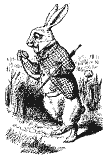
\includegraphics{RabbitWatch}\\
    \textbf{White Rabbit checking watch}
\end{center}

\noindent{The rabbit-hole went straight on like a tunnel for some way, and then dipped suddenly down, so suddenly that Alice had not a moment to think about stopping herself before she found herself falling down a very deep well.}

Either the well was very deep, or she fell very slowly, for she had plenty of time as she went down to look about her and to wonder what was going to happen next. First, she tried to look down and make out what she was coming to, but it was too dark to see anything; then she looked at the sides of the well, and noticed that they were filled with cupboards and book-shelves; here and there she saw maps and pictures hung upon pegs. She took down a jar from one of the shelves as she passed; it was labelled `ORANGE MARMALADE', but to her great disappointment it was empty: she did not like to drop the jar for fear of killing somebody, so managed to put it into one of the cupboards as she fell past it.

`Well!' thought Alice to herself, `after such a fall as this, I shall think nothing of tumbling down stairs! How brave they'll all think me at home! Why, I wouldn't say anything about it, even if I fell off the top of the house!' (Which was very likely true.)

Down, down, down. Would the fall never come to an end! `I wonder how many miles I've fallen by this time?' she said aloud. `I must be getting somewhere near the centre of the earth. Let me see: that would be four thousand miles down, I think--' (for, you see, Alice had learnt several things of this sort in her lessons in the schoolroom, and though this was not a very good opportunity for showing off her knowledge, as there was no one to listen to her, still it was good practice to say it over) `--yes, that's about the right distance--but then I wonder what Latitude or Longitude I've got to?' (Alice had no idea what Latitude was, or Longitude either, but thought they were nice grand words to say.)

Presently she began again. `I wonder if I shall fall right \textit{through} the earth! How funny it'll seem to come out among the people that walk with their heads downward! The Antipathies, I think--' (she was rather glad there was no one listening, this time, as it didn't sound at all the right word) `--but I shall have to ask them what the name of the country is, you know. Please, Ma'am, is this New Zealand or Australia?' (and she tried to curtsey as she spoke--fancy \textit{curtseying} as you're falling through the air! Do you think you could manage it?) `And what an ignorant little girl she'll think me for asking! No, it'll never do to ask: perhaps I shall see it written up somewhere.'

Down, down, down. There was nothing else to do, so Alice soon began talking again. `Dinah'll miss me very much to-night, I should think!' (Dinah was the cat.) `I hope they'll remember her saucer of milk at tea-time. Dinah my dear! I wish you were down here with me! There are no mice in the air, I'm afraid, but you might catch a bat, and that's very like a mouse, you know. But do cats eat bats, I wonder?' And here Alice began to get rather sleepy, and went on saying to herself, in a dreamy sort of way, `Do cats eat bats? Do cats eat bats?' and sometimes, `Do bats eat cats?' for, you see, as she couldn't answer either question, it didn't much matter which way she put it. She felt that she was dozing off, and had just begun to dream that she was walking hand in hand with Dinah, and saying to her very earnestly, `Now, Dinah, tell me the truth: did you ever eat a bat?' when suddenly, thump! thump! down she came upon a heap of sticks and dry leaves, and the fall was over.

Alice was not a bit hurt, and she jumped up on to her feet in a moment: she looked up, but it was all dark overhead; before her was another long passage, and the White Rabbit was still in sight, hurrying down it. There was not a moment to be lost: away went Alice like the wind, and was just in time to hear it say, as it turned a corner, `Oh my ears and whiskers, how late it's getting!' She was close behind it when she turned the corner, but the Rabbit was no longer to be seen: she found herself in a long, low hall, which was lit up by a row of lamps hanging from the roof.

There were doors all round the hall, but they were all locked; and when Alice had been all the way down one side and up the other, trying every door, she walked sadly down the middle, wondering how she was ever to get out again.

Suddenly she came upon a little three-legged table, all made of solid glass; there was nothing on it except a tiny golden key, and Alice's first thought was that it might belong to one of the doors of the hall; but, alas! either the locks were too large, or the key was too small, but at any rate it would not open any of them. However, on the second time round, she came upon a low curtain she had not noticed before, and behind it was a little door about fifteen inches high: she tried the little golden key in the lock, and to her great delight it fitted!

\begin{center}
    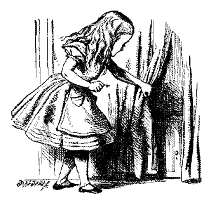
\includegraphics{TinyDoor}\\
    \textbf{Alice finding tiny door behind curtain\\}
\end{center}

\noindent{Alice opened the door and found that it led into a small passage, not much larger than a rat-hole: she knelt down and looked along the passage into the loveliest garden you ever saw. How she longed to get out of that dark hall, and wander about among those beds of bright flowers and those cool fountains, but she could not even get her head though the doorway; `and even if my head would go through,' thought poor Alice, `it would be of very little use without my shoulders. Oh, how I wish I could shut up like a telescope! I think I could, if I only know how to begin.' For, you see, so many out-of-the-way things had happened lately, that Alice had begun to think that very few things indeed were really impossible.}

There seemed to be no use in waiting by the little door, so she went back to the table, half hoping she might find another key on it, or at any rate a book of rules for shutting people up like telescopes: this time she found a little bottle on it, (`which certainly was not here before,' said Alice,) and round the neck of the bottle was a paper label, with the words `DRINK ME' beautifully printed on it in large letters.

\begin{center}
    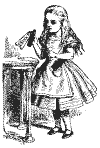
\includegraphics{DrinkMe}\\
    \textbf{Alice taking “Drink Me" bottle}
\end{center}

\noindent{It was all very well to say `Drink me,' but the wise little Alice was not going to do that in a hurry. `No, I'll look first,' she said, `and see whether it's marked "poison" or not'; for she had read several nice little histories about children who had got burnt, and eaten up by wild beasts and other unpleasant things, all because they would not remember the simple rules their friends had taught them: such as, that a red-hot poker will burn you if you hold it too long; and that if you cut your finger very deeply with a knife, it usually bleeds; and she had never forgotten that, if you drink much from a bottle marked `poison,' it is almost certain to disagree with you, sooner or later.}

However, this bottle was not marked `poison,' so Alice ventured to taste it, and finding it very nice, (it had, in fact, a sort of mixed flavour of cherry-tart, custard, pine-apple, roast turkey, toffee, and hot buttered toast,) she very soon finished it off.

\begin{center}
    * * *
\end{center}

\noindent{`What a curious feeling!' said Alice; `I must be shutting up like a telescope.'}
And so it was indeed: she was now only ten inches high, and her face brightened up at the thought that she was now the right size for going through the little door into that lovely garden. First, however, she waited for a few minutes to see if she was going to shrink any further: she felt a little nervous about this; `for it might end, you know,' said Alice to herself, `in my going out altogether, like a candle. I wonder what I should be like then?' And she tried to fancy what the flame of a candle is like after the candle is blown out, for she could not remember ever having seen such a thing.

After a while, finding that nothing more happened, she decided on going into the garden at once; but, alas for poor Alice! when she got to the door, she found she had forgotten the little golden key, and when she went back to the table for it, she found she could not possibly reach it: she could see it quite plainly through the glass, and she tried her best to climb up one of the legs of the table, but it was too slippery; and when she had tired herself out with trying, the poor little thing sat down and cried.

`Come, there's no use in crying like that!' said Alice to herself, rather sharply; `I advise you to leave off this minute!' She generally gave herself very good advice, (though she very seldom followed it), and sometimes she scolded herself so severely as to bring tears into her eyes; and once she remembered trying to box her own ears for having cheated herself in a game of croquet she was playing against herself, for this curious child was very fond of pretending to be two people. `But it's no use now,' thought poor Alice, `to pretend to be two people! Why, there's hardly enough of me left to make one respectable person!'

Soon her eye fell on a little glass box that was lying under the table: she opened it, and found in it a very small cake, on which the words `EAT ME' were beautifully marked in currants. `Well, I'll eat it,' said Alice, `and if it makes me grow larger, I can reach the key; and if it makes me grow smaller, I can creep under the door; so either way I'll get into the garden, and I don't care which happens!'

She ate a little bit, and said anxiously to herself, `Which way? Which way?', holding her hand on the top of her head to feel which way it was growing, and she was quite surprised to find that she remained the same size: to be sure, this generally happens when one eats cake, but Alice had got so much into the way of expecting nothing but out-of-the-way things to happen, that it seemed quite dull and stupid for life to go on in the common way.

So she set to work, and very soon finished off the cake.

\newpage

\section*{CHAPTER II \\ The Pool of Tears}

`Curiouser and curiouser!' cried Alice (she was so much surprised, that for the moment she quite forgot how to speak good English); `now I'm opening out like the largest telescope that ever was! Good-bye, feet!' (for when she looked down at her feet, they seemed to be almost out of sight, they were getting so far off). `Oh, my poor little feet, I wonder who will put on your shoes and stockings for you now, dears? I'm sure I shan't be able! I shall be a great deal too far off to trouble myself about you: you must manage the best way you can; --but I must be kind to them,' thought Alice, `or perhaps they won't walk the way I want to go! Let me see: I'll give them a new pair of boots every Christmas.'

\begin{center}
    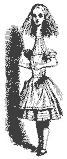
\includegraphics{AliceTall}\\
    \textbf{Alice stretched tall}
\end{center}

\noindent{And she went on planning to herself how she would manage it. `They must go by the carrier,' she thought; `and how funny it'll seem, sending presents to one's own feet! And how odd the directions will look!}

\begin{verse}

\texttt{ALICE'S RIGHT FOOT, ESQ.}\\
\hspace{1em}\texttt{HEARTHRUG,}\\
\hspace{2em}\texttt{NEAR THE FENDER,}\\
\hspace{3em}\texttt{(WITH ALICE'S LOVE).}

\end{verse}

\noindent{Oh dear, what nonsense I'm talking!'}

Just then her head struck against the roof of the hall: in fact she was now more than nine feet high, and she at once took up the little golden key and hurried off to the garden door.

Poor Alice! It was as much as she could do, lying down on one side, to look through into the garden with one eye; but to get through was more hopeless than ever: she sat down and began to cry again.

`You ought to be ashamed of yourself,' said Alice, `a great girl like you,' (she might well say this), `to go on crying in this way! Stop this moment, I tell you!' But she went on all the same, shedding gallons of tears, until there was a large pool all round her, about four inches deep and reaching half down the hall.

After a time she heard a little pattering of feet in the distance, and she hastily dried her eyes to see what was coming. It was the White Rabbit returning, splendidly dressed, with a pair of white kid gloves in one hand and a large fan in the other: he came trotting along in a great hurry, muttering to himself as he came, `Oh! the Duchess, the Duchess! Oh! won't she be savage if I've kept her waiting!' Alice felt so desperate that she was ready to ask help of any one; so, when the Rabbit came near her, she began, in a low, timid voice, `If you please, sir--' The Rabbit started violently, dropped the white kid gloves and the fan, and skurried away into the darkness as hard as he could go.

\begin{center}
    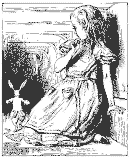
\includegraphics{RabbitRun}\\
    \textbf{Giant Alice watching Rabbit run away}
\end{center}

\noindent{Alice took up the fan and gloves, and, as the hall was very hot, she kept fanning herself all the time she went on talking: `Dear, dear! How queer everything is to-day! And yesterday things went on just as usual. I wonder if I've been changed in the night? Let me think: was I the same when I got up this morning? I almost think I can remember feeling a little different. But if I'm not the same, the next question is, Who in the world am I? Ah, \textit{that's} the great puzzle!' And she began thinking over all the children she knew that were of the same age as herself, to see if she could have been changed for any of them.}

`I'm sure I'm not Ada,' she said, `for her hair goes in such long ringlets, and mine doesn't go in ringlets at all; and I'm sure I can't be Mabel, for I know all sorts of things, and she, oh! she knows such a very little! Besides, \textit{she's} she, and I'm I, and--oh dear, how puzzling it all is! I'll try if I know all the things I used to know. Let me see: four times five is twelve, and four times six is thirteen, and four times seven is--oh dear! I shall never get to twenty at that rate! However, the Multiplication Table doesn't signify: let's try Geography. London is the capital of Paris, and Paris is the capital of Rome, and Rome--no, \textit{that's} all wrong, I'm certain! I must have been changed for Mabel! I'll try and say "How doth the little--"' and she crossed her hands on her lap as if she were saying lessons, and began to repeat it, but her voice sounded hoarse and strange, and the words did not come the same as they used to do:--

\newpage

\begin{verse}

\texttt{`How doth the little crocodile}\\
\hspace{1em}\texttt{Improve his shining tail,}\\
\texttt{And pour the waters of the Nile}\\
\hspace{1em}\texttt{On every golden scale!}\\

\end{verse}
\begin{verse}

\texttt{`How cheerfully he seems to grin,}\\
\hspace{1em}\texttt{How neatly spread his claws,}\\
\texttt{And welcome little fishes in}\\
\hspace{1em}\texttt{With gently smiling jaws!'}

\end{verse}

\noindent{`I'm sure those are not the right words,' said poor Alice, and her eyes filled with tears again as she went on, `I must be Mabel after all, and I shall have to go and live in that poky little house, and have next to no toys to play with, and oh! ever so many lessons to learn! No, I've made up my mind about it; if I'm Mabel, I'll stay down here! It'll be no use their putting their heads down and saying "Come up again, dear!" I shall only look up and say "Who am I then? Tell me that first, and then, if I like being that person, I'll come up: if not, I'll stay down here till I'm somebody else"--but, oh dear!' cried Alice, with a sudden burst of tears, `I do wish they \textit{would} put their heads down! I am so \textit{very} tired of being all alone here!'

As she said this she looked down at her hands, and was surprised to see that she had put on one of the Rabbit's little white kid gloves while she was talking. `How \textit{can} I have done that?' she thought. `I must be growing small again.' She got up and went to the table to measure herself by it, and found that, as nearly as she could guess, she was now about two feet high, and was going on shrinking rapidly: she soon found out that the cause of this was the fan she was holding, and she dropped it hastily, just in time to avoid shrinking away altogether.}

`That \textit{was} a narrow escape!' said Alice, a good deal frightened at the sudden change, but very glad to find herself still in existence; `and now for the garden!' and she ran with all speed back to the little door: but, alas! the little door was shut again, and the little golden key was lying on the glass table as before, `and things are worse than ever,' thought the poor child, `for I never was so small as this before, never! And I declare it's too bad, that it is!'

As she said these words her foot slipped, and in another moment, splash! she was up to her chin in salt water. Her first idea was that she had somehow fallen into the sea, `and in that case I can go back by railway,' she said to herself. (Alice had been to the seaside once in her life, and had come to the general conclusion, that wherever you go to on the English coast you find a number of bathing machines in the sea, some children digging in the sand with wooden spades, then a row of lodging houses, and behind them a railway station.) However, she soon made out that she was in the pool of tears which she had wept when she was nine feet high.

\begin{center}
    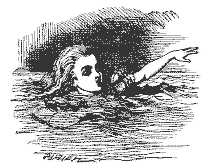
\includegraphics{AliceTears}\\
    \textbf{ Alice in pool of tears}
\end{center}

\noindent{`I wish I hadn't cried so much!' said Alice, as she swam about, trying to find her way out. `I shall be punished for it now, I suppose, by being drowned in my own tears! That will be a queer thing, to be sure! However, everything is queer to-day.'}

Just then she heard something splashing about in the pool a little way off, and she swam nearer to make out what it was: at first she thought it must be a walrus or hippopotamus, but then she remembered how small she was now, and she soon made out that it was only a mouse that had slipped in like herself.

\begin{center}
    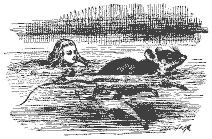
\includegraphics{AliceMouseTears}\\
    \textbf{Alice with Mouse in pool of tears}
\end{center}

\noindent{`Would it be of any use, now,' thought Alice, `to speak to this mouse? Everything is so out-of-the-way down here, that I should think very likely it can talk: at any rate, there's no harm in trying.' So she began: `O Mouse, do you know the way out of this pool? I am very tired of swimming about here, O Mouse!' (Alice thought this must be the right way of speaking to a mouse: she had never done such a thing before, but she remembered having seen in her brother's Latin Grammar, `A mouse--of a mouse--to a mouse--a mouse--O mouse!' The Mouse looked at her rather inquisitively, and seemed to her to wink with one of its little eyes, but it said nothing.}

`Perhaps it doesn't understand English,' thought Alice; `I daresay it's a French mouse, come over with William the Conqueror.' (For, with all her knowledge of history, Alice had no very clear notion how long ago anything had happened.) So she began again: `Ou est ma chatte?' which was the first sentence in her French lesson-book. The Mouse gave a sudden leap out of the water, and seemed to quiver all over with fright. `Oh, I beg your pardon!' cried Alice hastily, afraid that she had hurt the poor animal's feelings. `I quite forgot you didn't like cats.'

`Not like cats!' cried the Mouse, in a shrill, passionate voice. `Would you like cats if you were me?'

`Well, perhaps not,' said Alice in a soothing tone: `don't be angry about it. And yet I wish I could show you our cat Dinah: I think you'd take a fancy to cats if you could only see her. She is such a dear quiet thing,' Alice went on, half to herself, as she swam lazily about in the pool, `and she sits purring so nicely by the fire, licking her paws and washing her face--and she is such a nice soft thing to nurse--and she's such a capital one for catching mice--oh, I beg your pardon!' cried Alice again, for this time the Mouse was bristling all over, and she felt certain it must be really offended. `We won't talk about her any more if you'd rather not.'

`We indeed!' cried the Mouse, who was trembling down to the end of his tail. `As if I would talk on such a subject! Our family always hated cats: nasty, low, vulgar things! Don't let me hear the name again!'

`I won't indeed!' said Alice, in a great hurry to change the subject of conversation. `Are you--are you fond--of--of dogs?' The Mouse did not answer, so Alice went on eagerly: `There is such a nice little dog near our house I should like to show you! A little bright-eyed terrier, you know, with oh, such long curly brown hair! And it'll fetch things when you throw them, and it'll sit up and beg for its dinner, and all sorts of things--I can't remember half of them--and it belongs to a farmer, you know, and he says it's so useful, it's worth a hundred pounds! He says it kills all the rats and--oh dear!' cried Alice in a sorrowful tone, `I'm afraid I've offended it again!' For the Mouse was swimming away from her as hard as it could go, and making quite a commotion in the pool as it went.

So she called softly after it, `Mouse dear! Do come back again, and we won't talk about cats or dogs either, if you don't like them!' When the Mouse heard this, it turned round and swam slowly back to her: its face was quite pale (with passion, Alice thought), and it said in a low trembling voice, `Let us get to the shore, and then I'll tell you my history, and you'll understand why it is I hate cats and dogs.'

It was high time to go, for the pool was getting quite crowded with the birds and animals that had fallen into it: there were a Duck and a Dodo, a Lory and an Eaglet, and several other curious creatures. Alice led the way, and the whole party swam to the shore.

\newpage

\section*{CHAPTER III \\ A Caucus-Race and a Long Tale}

\noindent{They were indeed a queer-looking party that assembled on the bank--the birds with draggled feathers, the animals with their fur clinging close to them, and all dripping wet, cross, and uncomfortable.}

The first question of course was, how to get dry again: they had a consultation about this, and after a few minutes it seemed quite natural to Alice to find herself talking familiarly with them, as if she had known them all her life. Indeed, she had quite a long argument with the Lory, who at last turned sulky, and would only say, `I am older than you, and must know better'; and this Alice would not allow without knowing how old it was, and, as the Lory positively refused to tell its age, there was no more to be said.

At last the Mouse, who seemed to be a person of authority among them, called out, `Sit down, all of you, and listen to me! I'll soon make you dry enough!' They all sat down at once, in a large ring, with the Mouse in the middle. Alice kept her eyes anxiously fixed on it, for she felt sure she would catch a bad cold if she did not get dry very soon.

`Ahem!' said the Mouse with an important air, `are you all ready? This is the driest thing I know. Silence all round, if you please! "William the Conqueror, whose cause was favoured by the pope, was soon submitted to by the English, who wanted leaders, and had been of late much accustomed to usurpation and conquest. Edwin and Morcar, the earls of Mercia and Northumbria--"'

`Ugh!' said the Lory, with a shiver.

`I beg your pardon!' said the Mouse, frowning, but very politely: `Did you speak?'

`Not I!' said the Lory hastily.

`I thought you did,' said the Mouse. `--I proceed. "Edwin and Morcar, the earls of Mercia and Northumbria, declared for him: and even Stigand, the patriotic archbishop of Canterbury, found it advisable--"'

`Found what?' said the Duck.

`Found it,' the Mouse replied rather crossly: `of course you know what "it" means.'

`I know what "it" means well enough, when I find a thing,' said the Duck: `it's generally a frog or a worm. The question is, what did the archbishop find?'

The Mouse did not notice this question, but hurriedly went on, `"--found it advisable to go with Edgar Atheling to meet William and offer him the crown. William's conduct at first was moderate. But the insolence of his Normans--" How are you getting on now, my dear?' it continued, turning to Alice as it spoke.

`As wet as ever,' said Alice in a melancholy tone: `it doesn't seem to dry me at all.'

`In that case,' said the Dodo solemnly, rising to its feet, `I move that the meeting adjourn, for the immediate adoption of more energetic remedies--'

`Speak English!' said the Eaglet. `I don't know the meaning of half those long words, and, what's more, I don't believe you do either!' And the Eaglet bent down its head to hide a smile: some of the other birds tittered audibly.

`What I was going to say,' said the Dodo in an offended tone, `was, that the best thing to get us dry would be a Caucus-race.'

`What is a Caucus-race?' said Alice; not that she wanted much to know, but the Dodo had paused as if it thought that somebody ought to speak, and no one else seemed inclined to say anything.

`Why,' said the Dodo, `the best way to explain it is to do it.' (And, as you might like to try the thing yourself, some winter day, I will tell you how the Dodo managed it.)

First it marked out a race-course, in a sort of circle, (`the exact shape doesn't matter,' it said,) and then all the party were placed along the course, here and there. There was no `One, two, three, and away,' but they began running when they liked, and left off when they liked, so that it was not easy to know when the race was over. However, when they had been running half an hour or so, and were quite dry again, the Dodo suddenly called out `The race is over!' and they all crowded round it, panting, and asking, `But who has won?'

This question the Dodo could not answer without a great deal of thought, and it sat for a long time with one finger pressed upon its forehead (the position in which you usually see Shakespeare, in the pictures of him), while the rest waited in silence. At last the Dodo said, `Everybody has won, and all must have prizes.'

`But who is to give the prizes?' quite a chorus of voices asked.

`Why, she, of course,' said the Dodo, pointing to Alice with one finger; and the whole party at once crowded round her, calling out in a confused way, `Prizes! Prizes!'

Alice had no idea what to do, and in despair she put her hand in her pocket, and pulled out a box of comfits, (luckily the salt water had not got into it), and handed them round as prizes. There was exactly one a-piece all round.

`But she must have a prize herself, you know,' said the Mouse.

`Of course,' the Dodo replied very gravely. `What else have you got in your pocket?' he went on, turning to Alice.

`Only a thimble,' said Alice sadly.

`Hand it over here,' said the Dodo.

Then they all crowded round her once more, while the Dodo solemnly presented the thimble, saying `We beg your acceptance of this elegant thimble'; and, when it had finished this short speech, they all cheered.

\begin{center}
    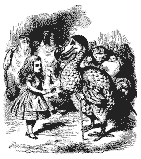
\includegraphics{DodoThimble}\\
    \textbf{Dodo presenting thimble}
\end{center}

\noindent{Alice thought the whole thing very absurd, but they all looked so grave that she did not dare to laugh; and, as she could not think of anything to say, she simply bowed, and took the thimble, looking as solemn as she could.}

The next thing was to eat the comfits: this caused some noise and confusion, as the large birds complained that they could not taste theirs, and the small ones choked and had to be patted on the back. However, it was over at last, and they sat down again in a ring, and begged the Mouse to tell them something more.

`You promised to tell me your history, you know,' said Alice, `and why it is you hate--C and D,' she added in a whisper, half afraid that it would be offended again.

`Mine is a long and a sad tale!' said the Mouse, turning to Alice, and sighing.

`It is a long tail, certainly,' said Alice, looking down with wonder at the Mouse's tail; `but why do you call it sad?' And she kept on puzzling about it while the Mouse was speaking, so that her idea of the tale was something like this:--

\begin{verse}

\hspace{3em}\texttt{`Fury said to a}\\
\hspace{2.8em}\texttt{mouse, That he}\\
\hspace{1.5em}\texttt{met in the}\\
\hspace{1em}\texttt{house,}\\
\hspace{0em}\texttt{"Let us}\\
\hspace{1em}\texttt{both go to}\\
\hspace{1.8em}\texttt{law:  I will}\\
                  prosecute\\
                    YOU.  --Come,\\
                       I'll take no\\
                        denial; We\\
                     must have a\\
                 trial:  For\\
              really this\\
\end{verse}

\begin{verse}

           morning I've
          nothing
         to do."
         
\end{verse}

\begin{verse}

           Said the
             mouse to the
               cur, "Such
                 a trial,
                   dear Sir,
                         With
                     no jury
                  or judge,
                would be
              wasting
             our
              breath."
               "I'll be
                 judge, I'll
                   be jury,"
                         Said
                    cunning
                      old Fury:
                     "I'll
                      try the
                         whole
                          cause,
                             and
                        condemn
                       you
                      to
                       death."'
\end{verse}                      
                       
\noindent{`You are not attending!' said the Mouse to Alice severely. `What are you thinking of?'}

\begin{center}
    \includegraphics{MouseStory}\\
    \textbf{Mouse telling story to birds and Alice}
\end{center}

\noindent{`I beg your pardon,' said Alice very humbly: `you had got to the fifth bend, I think?'}

`I had not!' cried the Mouse, sharply and very angrily.

`A knot!' said Alice, always ready to make herself useful, and looking anxiously about her. `Oh, do let me help to undo it!'

`I shall do nothing of the sort,' said the Mouse, getting up and walking away. `You insult me by talking such nonsense!'

`I didn't mean it!' pleaded poor Alice. `But you're so easily offended, you know!'

The Mouse only growled in reply.

`Please come back and finish your story!' Alice called after it; and the others all joined in chorus, `Yes, please do!' but the Mouse only shook its head impatiently, and walked a little quicker.

`What a pity it wouldn't stay!' sighed the Lory, as soon as it was quite out of sight; and an old Crab took the opportunity of saying to her daughter `Ah, my dear! Let this be a lesson to you never to lose your temper!' `Hold your tongue, Ma!' said the young Crab, a little snappishly. `You're enough to try the patience of an oyster!'

`I wish I had our Dinah here, I know I do!' said Alice aloud, addressing nobody in particular. `She'd soon fetch it back!'

`And who is Dinah, if I might venture to ask the question?' said the Lory.

Alice replied eagerly, for she was always ready to talk about her pet: `Dinah's our cat. And she's such a capital one for catching mice you can't think! And oh, I wish you could see her after the birds! Why, she'll eat a little bird as soon as look at it!'

This speech caused a remarkable sensation among the party. Some of the birds hurried off at once: one old Magpie began wrapping itself up very carefully, remarking, `I really must be getting home; the night-air doesn't suit my throat!' and a Canary called out in a trembling voice to its children, `Come away, my dears! It's high time you were all in bed!' On various pretexts they all moved off, and Alice was soon left alone.

`I wish I hadn't mentioned Dinah!' she said to herself in a melancholy tone. `Nobody seems to like her, down here, and I'm sure she's the best cat in the world! Oh, my dear Dinah! I wonder if I shall ever see you any more!' And here poor Alice began to cry again, for she felt very lonely and low-spirited. In a little while, however, she again heard a little pattering of footsteps in the distance, and she looked up eagerly, half hoping that the Mouse had changed his mind, and was coming back to finish his story.

\end{document}